\documentclass[11pt]{article}

\usepackage[colorlinks=true]{hyperref}

% This is a toggle for whether the solutions should be included in output of this document
\newif\ifSolutions
%\Solutionsfalse  % this is used to exclude the solutions
\Solutionstrue  % this is used to include the solutions


\usepackage[left=0.8in, right=0.8in, top=0.7in, bottom=1in, includefoot]{geometry}
\usepackage{fancyhdr}
\usepackage{array}
\usepackage{multicol}
\setlength{\parindent}{0mm}
\setlength{\parskip}{5pt}
\usepackage{sectsty}
\allsectionsfont{\sffamily}
\setlength{\headheight}{2cm}
\usepackage{amsmath,amssymb,bm}
\usepackage{booktabs}
\usepackage{graphicx}
\usepackage{color}
\usepackage{cancel}
\usepackage{comment}
\usepackage{hyperref}
\usepackage{subfig}
\usepackage{multirow}
\usepackage{placeins}

% Global definitions
%
% boldface letters
%
%\newcommand{\boldface}[1]{\mathbf{#1}}   % upright
\newcommand{\boldface}[1]{\boldsymbol{#1}}  % italic (slanted)
%
\newcommand{\bfa}{\boldface{a}}
\newcommand{\bfb}{\boldface{b}}
\newcommand{\bfc}{\boldface{c}}
\newcommand{\bfd}{\boldface{d}}
\newcommand{\bfe}{\boldface{e}}
\newcommand{\bff}{\boldface{f}}
\newcommand{\bfg}{\boldface{g}}
\newcommand{\bfh}{\boldface{h}}
\newcommand{\bfi}{\boldface{i}}
\newcommand{\bfj}{\boldface{j}}
\newcommand{\bfk}{\boldface{k}}
\newcommand{\bfl}{\boldface{l}}
\newcommand{\bfm}{\boldface{m}}
\newcommand{\bfn}{\boldface{n}}
\newcommand{\bfo}{\boldface{o}}
\newcommand{\bfp}{\boldface{p}}
\newcommand{\bfq}{\boldface{q}}
\newcommand{\bfr}{\boldface{r}}
\newcommand{\bfs}{\boldface{s}}
\newcommand{\bft}{\boldface{t}}
\newcommand{\bfu}{\boldface{u}}
\newcommand{\bfv}{\boldface{v}}
\newcommand{\bfw}{\boldface{w}}
\newcommand{\bfx}{\boldface{x}}
\newcommand{\bfy}{\boldface{y}}
\newcommand{\bfz}{\boldface{z}}
%
\newcommand{\bfA}{\boldface{A}}
\newcommand{\bfB}{\boldface{B}}
\newcommand{\bfC}{\boldface{C}}
\newcommand{\bfD}{\boldface{D}}
\newcommand{\bfE}{\boldface{E}}
\newcommand{\bfF}{\boldface{F}}
\newcommand{\bfG}{\boldface{G}}
\newcommand{\bfH}{\boldface{H}}
\newcommand{\bfI}{\boldface{I}}
\newcommand{\bfJ}{\boldface{J}}
\newcommand{\bfK}{\boldface{K}}
\newcommand{\bfL}{\boldface{L}}
\newcommand{\bfM}{\boldface{M}}
\newcommand{\bfN}{\boldface{N}}
\newcommand{\bfO}{\boldface{O}}
\newcommand{\bfP}{\boldface{P}}
\newcommand{\bfQ}{\boldface{Q}}
\newcommand{\bfR}{\boldface{R}}
\newcommand{\bfS}{\boldface{S}}
\newcommand{\bfT}{\boldface{T}}
\newcommand{\bfU}{\boldface{U}}
\newcommand{\bfV}{\boldface{V}}
\newcommand{\bfW}{\boldface{W}}
\newcommand{\bfX}{\boldface{X}}
\newcommand{\bfY}{\boldface{Y}}
\newcommand{\bfZ}{\boldface{Z}}

\newcommand{\bfFe}{\boldface{F}_{\text{e}}}
\newcommand{\bfFp}{\boldface{F}_{\text{p}}}
\newcommand{\bfepse}{\pmb{\varepsilon}_{\text{e}}}
\newcommand{\bfepsp}{\pmb{\varepsilon}_{\text{p}}}
\newcommand{\bfeps}{\pmb{\varepsilon}}

%
% boldface greek symbols
%
\newcommand{\bfalpha}{\boldsymbol{\alpha}}
\newcommand{\bfbeta}{\boldsymbol{\beta}}
\newcommand{\bfgamma}{\boldsymbol{\gamma}}
\newcommand{\bfdelta}{\boldsymbol{\delta}}
\newcommand{\bfepsilon}{\pmb{\varepsilon}}
\newcommand{\bfzeta}{\boldsymbol{\zeta}}
\newcommand{\bfeta}{\boldsymbol{\eta}}
\newcommand{\bftheta}{\boldsymbol{\theta}}
\newcommand{\bfkappa}{\boldsymbol{\kappa}}
\newcommand{\bflambda}{\boldsymbol{\lambda}}
\newcommand{\bfrho}{\boldsymbol{\rho}}
\newcommand{\bfmu}{\boldsymbol{\mu}}
\newcommand{\bfnu}{\boldsymbol{\nu}}
\newcommand{\bfpi}{\boldsymbol{\pi}}
\newcommand{\bfxi}{\boldsymbol{\xi}}
\newcommand{\bfsigma}{\boldsymbol{\sigma}}
\newcommand{\bftau}{\boldsymbol{\tau}}
\newcommand{\bfphi}{\boldsymbol{\phi}}
\newcommand{\bfvarphi}{\boldsymbol{\varphi}}
\newcommand{\bfchi}{\boldsymbol{\chi}}
\newcommand{\bfomega}{\boldsymbol{\omega}}
\newcommand{\bfnull}{\boldsymbol{0}}
%
\newcommand{\bfGamma}{\boldsymbol{\Gamma}}
\newcommand{\bfDelta}{\boldsymbol{\Delta}}
\newcommand{\bfTheta}{\boldsymbol{\Theta}}
\newcommand{\bfLambda}{\boldsymbol{\Lambda}}
\newcommand{\bfPi}{\boldsymbol{\Pi}}
\newcommand{\bfXi}{\boldsymbol{\Xi}}
\newcommand{\bfSigma}{\boldsymbol{\Sigma}}
\newcommand{\bfPhi}{\boldsymbol{\Phi}}
\newcommand{\bfChi}{\boldsymbol{\Chi}}
\newcommand{\bfOmega}{\boldsymbol{\Omega}}
\newcommand{\bfnabla}{\boldsymbol{\nabla}}
\newcommand{\laplace}{\boldsymbol{\Delta}}
%
% caligraphic letters
%
\newcommand{\calA}{\mathcal{A}}
\newcommand{\calB}{\mathcal{B}}
\newcommand{\calC}{\mathcal{C}}
\newcommand{\calD}{\mathcal{D}}
\newcommand{\calE}{\mathcal{E}}
\newcommand{\calF}{\mathcal{F}}
\newcommand{\calG}{\mathcal{G}}
\newcommand{\calH}{\mathcal{H}}
\newcommand{\calI}{\mathcal{I}}
\newcommand{\calJ}{\mathcal{J}}
\newcommand{\calK}{\mathcal{K}}
\newcommand{\calL}{\mathcal{L}}
\newcommand{\calM}{\mathcal{M}}
\newcommand{\calN}{\mathcal{N}}
\newcommand{\calO}{\mathcal{O}}
\newcommand{\calP}{\mathcal{P}}
\newcommand{\calQ}{\mathcal{Q}}
\newcommand{\calR}{\mathbb{R}}
\newcommand{\calS}{\mathcal{S}}
\newcommand{\calT}{\mathcal{T}}
\newcommand{\calU}{\mathcal{U}}
\newcommand{\calV}{\mathcal{V}}
\newcommand{\calW}{\mathcal{W}}
\newcommand{\calX}{\mathcal{X}}
\newcommand{\calY}{\mathcal{Y}}
\newcommand{\calZ}{\mathcal{Z}}
% .. define more if needed
%
% double stroke
%
\newcommand{\dsA}{\mathbb{A}}
\newcommand{\dsB}{\mathbb{B}}
\newcommand{\dsC}{\mathbb{C}}
\newcommand{\dsD}{\mathbb{D}}
\newcommand{\dsE}{\mathbb{E}}
\newcommand{\dsF}{\mathbb{F}}
\newcommand{\dsG}{\mathbb{G}}
\newcommand{\dsH}{\mathbb{H}}
\newcommand{\dsI}{\mathbb{I}}
\newcommand{\dsJ}{\mathbb{J}}
\newcommand{\dsK}{\mathbb{K}}
\newcommand{\dsL}{\mathbb{L}}
\newcommand{\dsM}{\mathbb{M}}
\newcommand{\dsN}{\mathbb{N}}
\newcommand{\dsO}{\mathbb{O}}
\newcommand{\dsP}{\mathbb{P}}
\newcommand{\dsQ}{\mathbb{Q}}
\newcommand{\dsR}{\mathbb{R}}
\newcommand{\dsS}{\mathbb{S}}
\newcommand{\dsT}{\mathbb{T}}
\newcommand{\dsU}{\mathbb{U}}
\newcommand{\dsV}{\mathbb{V}}
\newcommand{\dsW}{\mathbb{W}}
\newcommand{\dsX}{\mathbb{X}}
\newcommand{\dsY}{\mathbb{Y}}
\newcommand{\dsZ}{\mathbb{Z}}



\newcommand{\vect}[1]{\mathbf{#1}}
\newcommand{\grvect}[1]{\mbox{\boldmath{$#1$}}}
\newcommand{\perm}{\mbox{{\Huge $\epsilon$}}}
\newcommand{\transvect}[1]{\vect{#1}^{\mbox{\footnotesize T}}}
\newcommand{\invvect}[1]{\vect{#1}^{\mbox{\footnotesize -1}}}
\newcommand{\partderiv}[2]{\frac{\partial #1}{\partial #2}}
\newcommand{\partderivv}[2]{\frac{\partial^2 #1}{\partial #2^2}}
\newcommand{\totalderiv}[2]{\frac{d #1}{d #2}}

\newcommand{\mg}[1]{{\boldsymbol{#1}}}
\newcommand{\mf}[1]{{\mathfrak{#1}}}
\newcommand{\mfb}[1]{{\boldsymbol{\mathfrak{#1}}}}
\newcommand{\ms}[1]{{\mathscr{#1}}}
\newcommand{\mb}[1]{{\mathbf{#1}}}
\newcommand{\mbb}[1]{{\mathbb{#1}}}
\newcommand{\mbbu}[1]{{\underline{\mathbb{#1}}}\vphantom{#1}}
\newcommand{\mbu}[1]{{\underline{\mathbf{#1}}}\vphantom{#1}}
\newcommand{\mgu}[1]{{\underline{\boldsymbol{#1}}}\vphantom{#1}}
\newcommand{\mr}[1]{{\mathrm{#1}}}
\newcommand{\msf}[1]{{\mathsf{#1}}}
\newcommand{\msfb}[1]{{\boldsymbol{\mathsf{#1}}}}

\newcommand{\dotprod}{\stackrel{\scriptscriptstyle \bullet}{}}
\newcommand{\half}{\frac{1}{2}}
\newcommand{\T}{^{\mathsf{T}}} % x^{T}
\newcommand{\mT}{^{\mathsf{-T}}} % x^{-T}
\newcommand{\wass}{\mathsf{wass}}
\newcommand{\eff}{\mathsf{eff}}
\newcommand{\me}{^{\mathrm{-1}}} % x^{-1}
\newcommand{\Rset}{\ensuremath{\mathbb{R}}}
\newcommand{\Kset}{\ensuremath{K}}
\newcommand{\bul}{$\bullet\;$}
%\newcommand{\red}{\mathrm{red}}
\newcommand{\Fe}{\mathbf{F}_\mathbf{e}}
\newcommand{\Fp}{\mathbf{F}_\mathbf{p}}
\def\rel{{\mathrm{rel}}}

%\newcommand{\D}{\displaystyle}
\newcommand{\abs}{\rule[-1cm]{0cm}{1cm}}
\newcommand{\babs}{\rule[-1cm]{0cm}{2cm}}

\newlength{\boxwidth}
\setlength{\boxwidth}{\textwidth}
\addtolength{\boxwidth}{-1cm}

\newcommand\pl{\partial}
\def\dd{\;\!\mathrm{d}}
\def\DD{\;\!\mathrm{D}}
\def\Lin{\R^{d\times d}} 
\def\R{I\!R}
\def\AM{{\mathrm{AM}}}

\def\btheorem{\begin{theorem}}
\def\etheorem{\end{theorem}}
\def\blemma{\begin{lemma}}
\def\elemma{\end{lemma}}
\def\bproposition{\begin{proposition}}
\def\eproposition{\end{proposition}}
\def\bcorollary{\begin{corollary}}
\def\ecorollary{\end{corollary}}
\def\bdefinition{\begin{definition}}
\def\edefinition{\end{definition}}
\def\bexample{\begin{example}}
\def\eexample{\end{example}}
\def\bremark{\begin{remark}}
\def\eremark{\end{remark}}
\def\bproblem#1{\medskip \noindent {\bf #1}\sl \\ }
\def\eproblem{\rm \medskip}
\newcommand{\bma}{ \left( \ba}
\newcommand{\ema}{ \ea \right)}
\newcommand{\set}[2]{\big\{\: #1 \: \big| \: #2 \:\big\} }
\def\cD{\mathcal{D}}
\def\cL{\mathcal{L}}
\def\cG{\mathcal{G}}
\def\cI{\mathcal{I}}
\def\cJ{\mathcal{J}}
\def\ccA{\mathcal{A}}
\def\rmD{\mathrm{D}}
\def\bbQ{\mathbb{Q}}
\def\bbA{\fg{A\!\!\!A}}
\def\fg{\boldsymbol}
\def\mdot{\fg{:}}
\def\vdot{\fg{\cdot}}
\newcommand{\el}{\mathsf{el}}
\def\id{{\bfI}}
\def\eqldef{{\:{\stackrel{\mathrm{def}}{=}}\:}}
\newcommand{\eps}{\varepsilon}
\def\ol{\overline}
\def\wt{\widetilde}
\def\wh{\widehat}
\def\ds{\displaystyle}
\def\ts{\textstyle}
\def\mtr{^\mathrm{-T}}
\def\inh{^\mathrm{inh}}
\DeclareMathOperator{\divv}{div}
\DeclareMathOperator{\grad}{grad}
\DeclareMathOperator{\tr}{tr}
\DeclareMathOperator{\curl}{curl}
\DeclareMathOperator{\Curl}{Curl}
%\DeclareMathOperator{\T}{T}
\DeclareMathOperator{\argmin}{{arg\,min}}
\DeclareMathOperator{\diag}{diag}
\DeclareMathOperator{\trace}{tr}
\DeclareMathOperator{\sign}{sign}
\DeclareMathOperator{\dev}{dev}
\DeclareMathOperator{\cof}{cof}
\DeclareMathOperator{\sym}{sym}
\DeclareMathOperator{\skews}{skw}
\def\Felast{\bfF_\mathbf{\!e}}
\def\Fplast{\bfF_\mathbf{\!p}}
\def\Cplast{\bfC_\mathbf{\!p}}
\def\epselast{\bfeps_\mathbf{\!e}}
\def\epsplast{\bfeps_\mathbf{\!p}}
\def\GLin{\mbox{{\sf GL}$(d)$}}  %{\R^{d\times d}_*}% invertible matrices
\def\Lin{\R^{d\times d}}        % all d times d matrices
\def\reff#1{(\ref{#1})}
\def\red{{\mathrm{red}}}
\def\rep{{\mathrm{rep}}}
\def\cond{{\mathrm{cond}}}
\newcommand{\kopfcolor}{\color{red}}
\newcommand{\er}{\hspace*{4cm}}
\newcommand{\n}{{\rm n}}
\newcommand{\nn}{{\rm n+1}}
\newcommand{\PsiS}{\Psi_\mathrm{S}}
\newcommand{\PsiV}{\Psi_\mathrm{V}}
\newcommand{\PsiI}{\Psi_\mathrm{I}}
\newcommand{\cA}{c_\mathrm{A}}
\newcommand{\cM}{c_\mathrm{M}}

\newcommand{\calAe}{\underset{e=1}{\overset{n_e}{\mathcal{A}}}}
\newcommand{\Grad}{\text{Grad}}
\newcommand{\tcr}{\tau_{\text{crit}}}
\newcommand{\be}{\begin{equation}\nonumber}
\newcommand{\ee}{\end{equation}}
\newcommand{\beq}{\begin{eqnarray}}
\newcommand{\eeq}{\end{eqnarray}}
\newcommand{\bem}{\begin{multline}}
\newcommand{\eem}{\end{multline}}
\newcommand{\ba}{\begin{align}}
\newcommand{\ea}{\end{align}}
\newcommand{\bfzero}{{\fg0}}

\renewcommand{\figurename}{Figure}
\renewcommand{\tablename}{Table}

\newcommand{\fp}[2]{\frac{\partial #1}{\partial #2} }
\newcommand{\LR}{{\qquad \Leftrightarrow \qquad }}
\newcounter{problem}
\newcounter{points}
\newcounter{stretchPoints}

\newcommand{\head}[3]{

\begin{center}
\section*{Homework Set \##1 \ifSolutions Solutions \fi}
assigned: #2\\
due: #3, 11:00 pm\\
in your repo at /cs/cs181j/2015/fall/students/your\_user\_name/cs181j \\
\end{center}
\hrule
\vskip 0.1cm
}

\newcommand{\prob}[1]{\par\vskip 0.5cm \stepcounter{problem}\subsubsection*{Problem \arabic{problem} \ \small (#1 points).}\addtocounter{points}{#1}}
\newcommand{\total}{
\begin{flushright}
\small\par\vskip 0.3cm \textit{total: \arabic{points} points ({\color{blue}+\arabic{stretchPoints} stretch points})}
\end{flushright}
}

\newcommand{\eprob}[2]{\par\vskip 0.5cm \stepcounter{problem}\subsubsection*{Problem \arabic{problem}: #2 \ \small (#1 points).}\addtocounter{points}{#1}}

\newcommand{\estretchprob}[3]{\par\vskip 0.5cm \stepcounter{problem}\subsubsection*{Problem \arabic{problem}: #3 \ \small (#1 points ({\color{blue}+#2 stretch points}) ).}\addtocounter{points}{#1}\addtocounter{stretchPoints}{#2}}


%\endinput

\usepackage{afterpage}
\usepackage{enumerate}

\begin{document}
\sffamily
\pagestyle{fancy}
\renewcommand{\headrulewidth}{0.4pt}
\fancyfoot[C]{\sffamily \thepage{}}
\fancyhead[C]{\vskip 0.7cm \sffamily\footnotesize \textbf{cs181j -- High Performance Computing} \hfill \name\\ Fall 2015 \hfill Harvey Mudd College}

% Convenience function used for including a figure
\newcommand\Figure[3]
{
    \begin{figure}[h!]
        \begin{center}
    \includegraphics[width=#3 in]{#1}
    \caption{\label{fig:#1} {#2}}
    \end{center}
    \end{figure}
}

\newcommand\TwoFigure[7]
{
    \begin{figure}[h!]
        \subfloat[#2]{\includegraphics[width=#7 in]{#1}}
    \hfill
        \subfloat[#4]{\includegraphics[width=#7 in]{#3}}
        \caption{\label{fig:#6}#5}
    \end{figure}
}

\newcommand\TwoFigureVertical[7]
{
    \begin{figure}[h!]
        \subfloat[#2]{\includegraphics[width=#7 in]{#1}}

        \subfloat[#4]{\includegraphics[width=#7 in]{#3}}
        \caption{\label{fig:#6}#5}
    \end{figure}
}


\fancyhead[RL]{}

%\newcommand{\name}{I forgot to change my name}


\head{10}{Friday, November 20, 2015}{Wednesday, November 25, 2015}

In this assignment, we'll continue exploring GPU programming though \href{http://docs.nvidia.com/cuda/cuda-c-programming-guide/}{cuda}.
Each problem has \texttt{cc}, \texttt{cuh}, and \texttt{cu} files.  
However, now that you've gone through the process of modifying the \texttt{cc} and \texttt{cuh} files on the previous assignment, I'll do all of that for you now; on this assignment you'll just write cuda kernels.
Remember that all problems are compared against a serial CPU version, so if you get a speedup of less than ~10, a threaded CPU version may go faster.








\eprob{15}{Breaking (Bad) Branches}

GPUs excel at doing independent calculations over many input values.  
We are going to test this by doing binary searches of many input values into a list of sorted integers.  
Binary searches are not ideal kernels for a GPU.  However, there's a lot of them and they're totally independent, so maybe the parallelism will win out.

You will implement a CPU and a GPU version of binary searching.  
You'll plot speedup with respect to the size of the input (number of searches you're making) table size (number of sorted integers in which you're searching for the inputs).  
So, if the input size is 1e6 and the table size is 1e2, then you will be making 1e6 searches into a list of 1e2 sorted numbers.

\begin{enumerate}[a)]
\item Implement the CPU version of (iterative, not recursive) binary searching (see, for example, \href{http://en.wikipedia.org/wiki/Binary_search_algorithm}{here}).  
Remember to handle the cases where the number you're searching for is greater than the last sorted number or less than the first.
Plot the \texttt{speedup} of your CPU version with respect to the \texttt{STL's binary\_search} function.  
How well do you perform?

\ifSolutions
\textbf{Solution}

\begin{center}

\includegraphics[width=3.50in, trim=1.25in .5in .75in 0.40in, clip]{figures/BinarySearch_cpu_shuffler}
\end{center}

\fi

\item Implement the GPU version of (iterative) binary searching.  
Remember to handle the edge cases!
Plot your \texttt{speedup} of your GPU version with respect to the \texttt{STL's binary\_search} function.  
How well do you perform?

\ifSolutions
\textbf{Solution}

{
  \begin{figure}[h!]
    \begin{center}
    \begin{tabular}{cc}
    \subfloat[log]{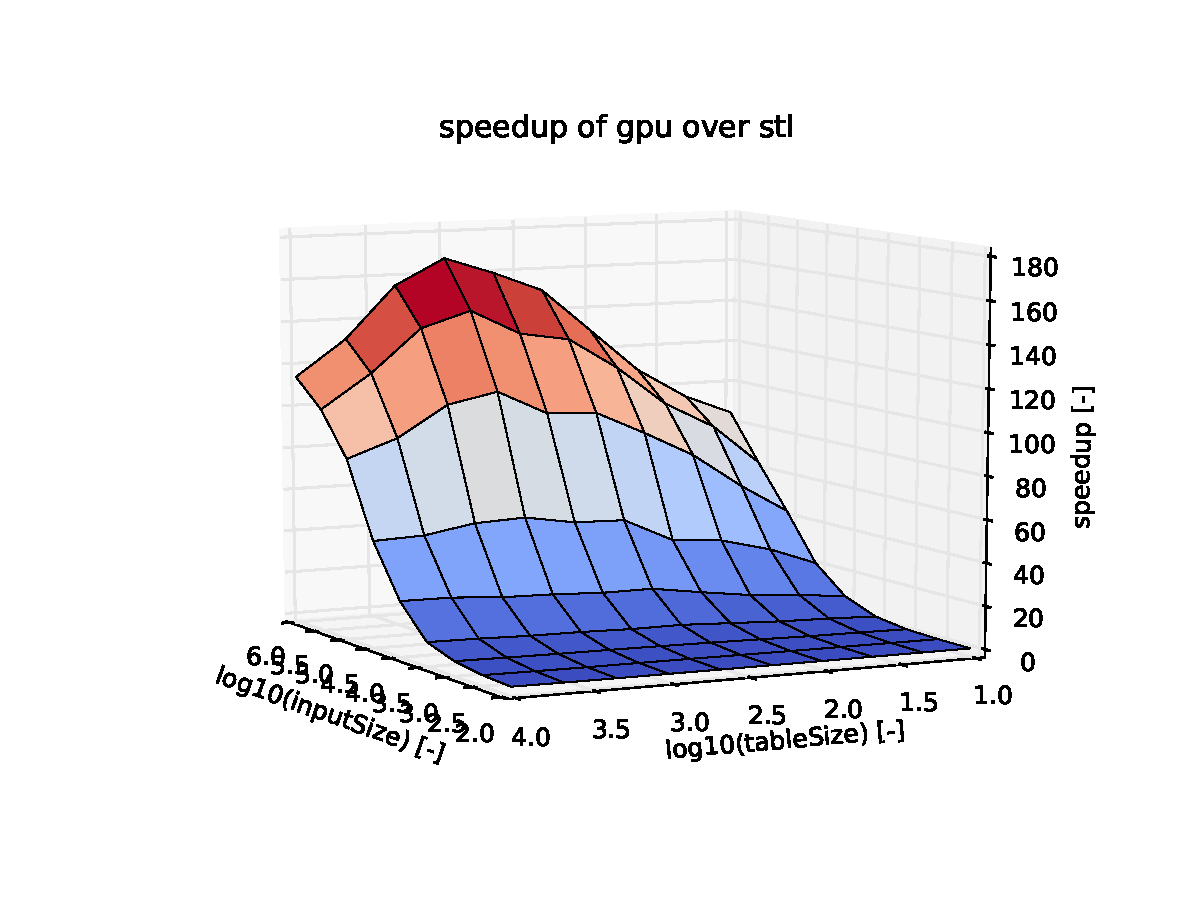
\includegraphics[width=3.00in, trim=1.25in .75in .75in 0.50in, clip]{figures/BinarySearch_gpu_linear_shuffler}} &
    \subfloat[linear]{
\includegraphics[width=3.00in, trim=1.25in .75in .75in 0.50in, clip]{figures/BinarySearch_gpu_log_shuffler}} \\
    \end{tabular}
    \end{center}
    \caption{Performance of binary searches on the GPU}
    \label{fig:BinarySearch}
  \end{figure}
}

\fi

\end{enumerate}

\FloatBarrier
\vfill




\eprob{20}{K-means GPU}

For this problem, we'll return to our recurring example of \href{https://en.wikipedia.org/wiki/K-means_clustering}{k-means clustering} (for a refresher on what it is, see homework 5).  
When threading for the CPU, the best technique was to duplicate the \texttt{nextCentroids} and \texttt{nextCentroidCounts} variables per thread and perform reductions.  
On the GPU, you may need to use an alternative strategy for coordinating between the threads.
Note that I have set up the provided code such that you'll work with points as Structure of Arrays instead of Array of Structures in your kernel, for maximum performance on the GPU.

Make a GPU version of the algorithm.  
How did you handle coordination between the threads?
The performance plot is included here; comment on what you see.  
When do you get good speedup?  Why?
  
\ifSolutions
\textbf{Solution:}
{
  \begin{figure}[ht]
    \begin{center}
    \begin{tabular}{cc}
    \subfloat[log]{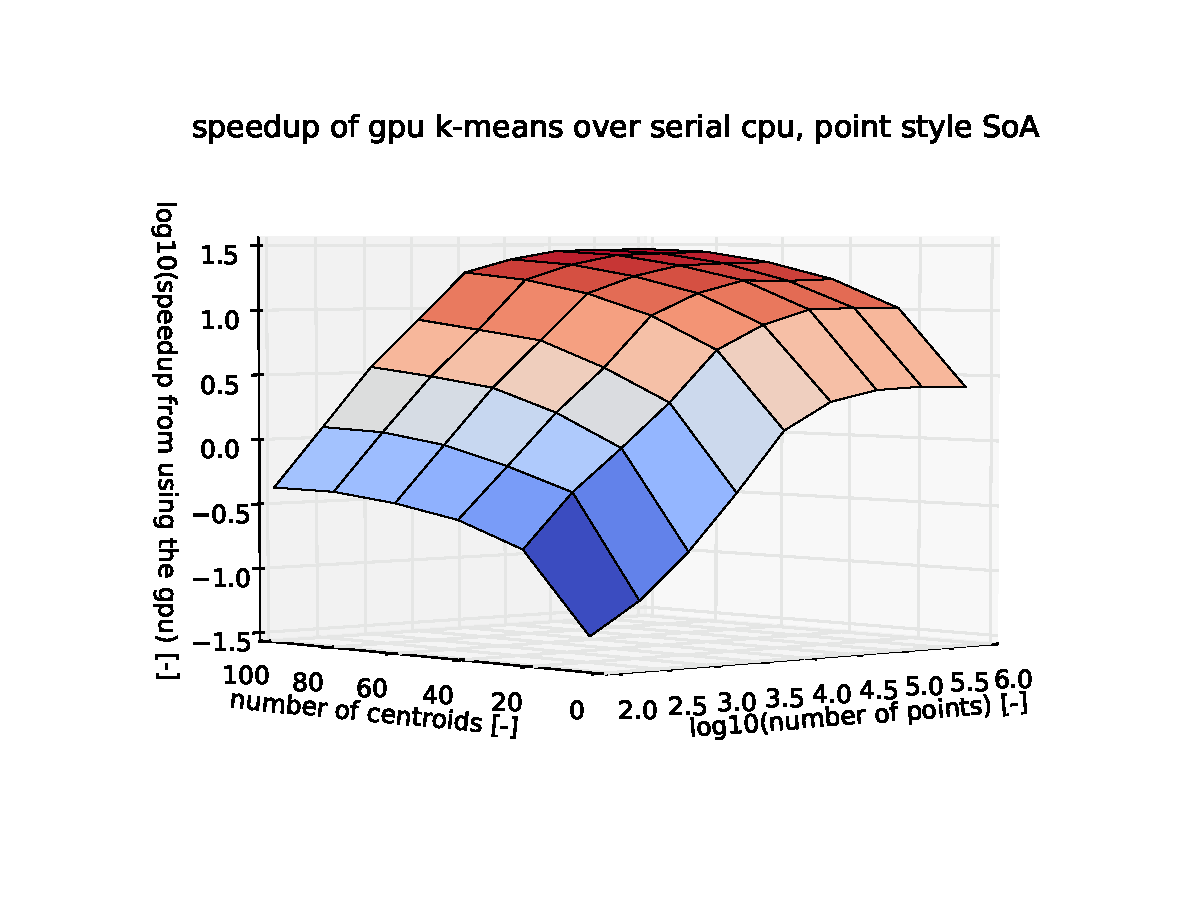
\includegraphics[width=3.0in, trim=1.0in .5in .75in .5in, clip]{figures/KMeansClustering_SoAVersusSerial_log_shuffler}} &
    \subfloat[linear]{
\includegraphics[width=3.0in, trim=1.0in .5in .75in .5in, clip]{figures/KMeansClustering_SoAVersusSerial_linear_shuffler}} \\
    \end{tabular}
    \end{center}
    \caption{Performance for KMeansClustering on the GPU}
    \label{fig:KMeansClustering}
  \end{figure}
}

\fi

\FloatBarrier
\vfill












\eprob{25}{Matrix Multiplication}

Matrix multiplication seems like a good candidate for using the GPU because it can have a high flop to data size ratio. 
In this problem, we'll re-do a couple of the ways of doing matrix multiplication that we've looked at in the past, but now on the GPU where segmentation faults are harder to find and life is more \textit{interesting}.  
We'll take standard row-major times row-major to be our baseline time.

In reality, if you just need to do \emph{one} multiplication of two matrices and you're thinking of using the GPU, you should just use GPU matrix library, such as \href{https://developer.nvidia.com/cublas}{cublas}.  
So, in this example we'll also compare our performance against \texttt{cublas' dgemm} \textbf{d}ouble precision \textbf{ge}neral \textbf{m}atrix \textbf{m}atrix multiplication function, but I've done all of that for you.

Implement the following three versions of matrix multiplication on the GPU:

\begin{enumerate}[1.]
\item The naive \texttt{rowMajor * rowMajor} version.  
This version was cache-unfriendly for the CPU and performs poorly there.
\item The naive \texttt{rowMajor * colMajor} version.  
This version was cache-friendly for the CPU and performed better there.
\item The row-major storage, tiled multiplication method from homework 3, where matrices are stored in row-major format but the actual multiplication is done with tiles. 
Each block is in charge of computing a whole tile in the output matrix, then strides by the number of blocks and keeps doing tiles until there are none left to do.
Use a fixed \texttt{numberOfThreadsPerBlock} of 1024 and a fixed \texttt{tileSize} of 32 (so that each thread in a block is handling one entry in the result matrix), and implement the following algorithm (illustrated in the figure below):

\begin{verbatim}
resultTileIndex = blockIndex
while (resultTileIndex < numberOfTiles)
  for dummyTile from 0 to numberOfTilesPerSide
    resultTiles(resultTileRow, resultTileCol) +=
      leftTiles(resultTileRow, dummyTile) * rightTiles(dummyTile, resultTileCol)
  resultTileIndex += numberOfBlocks
\end{verbatim}

\end{enumerate}

\begin{center}
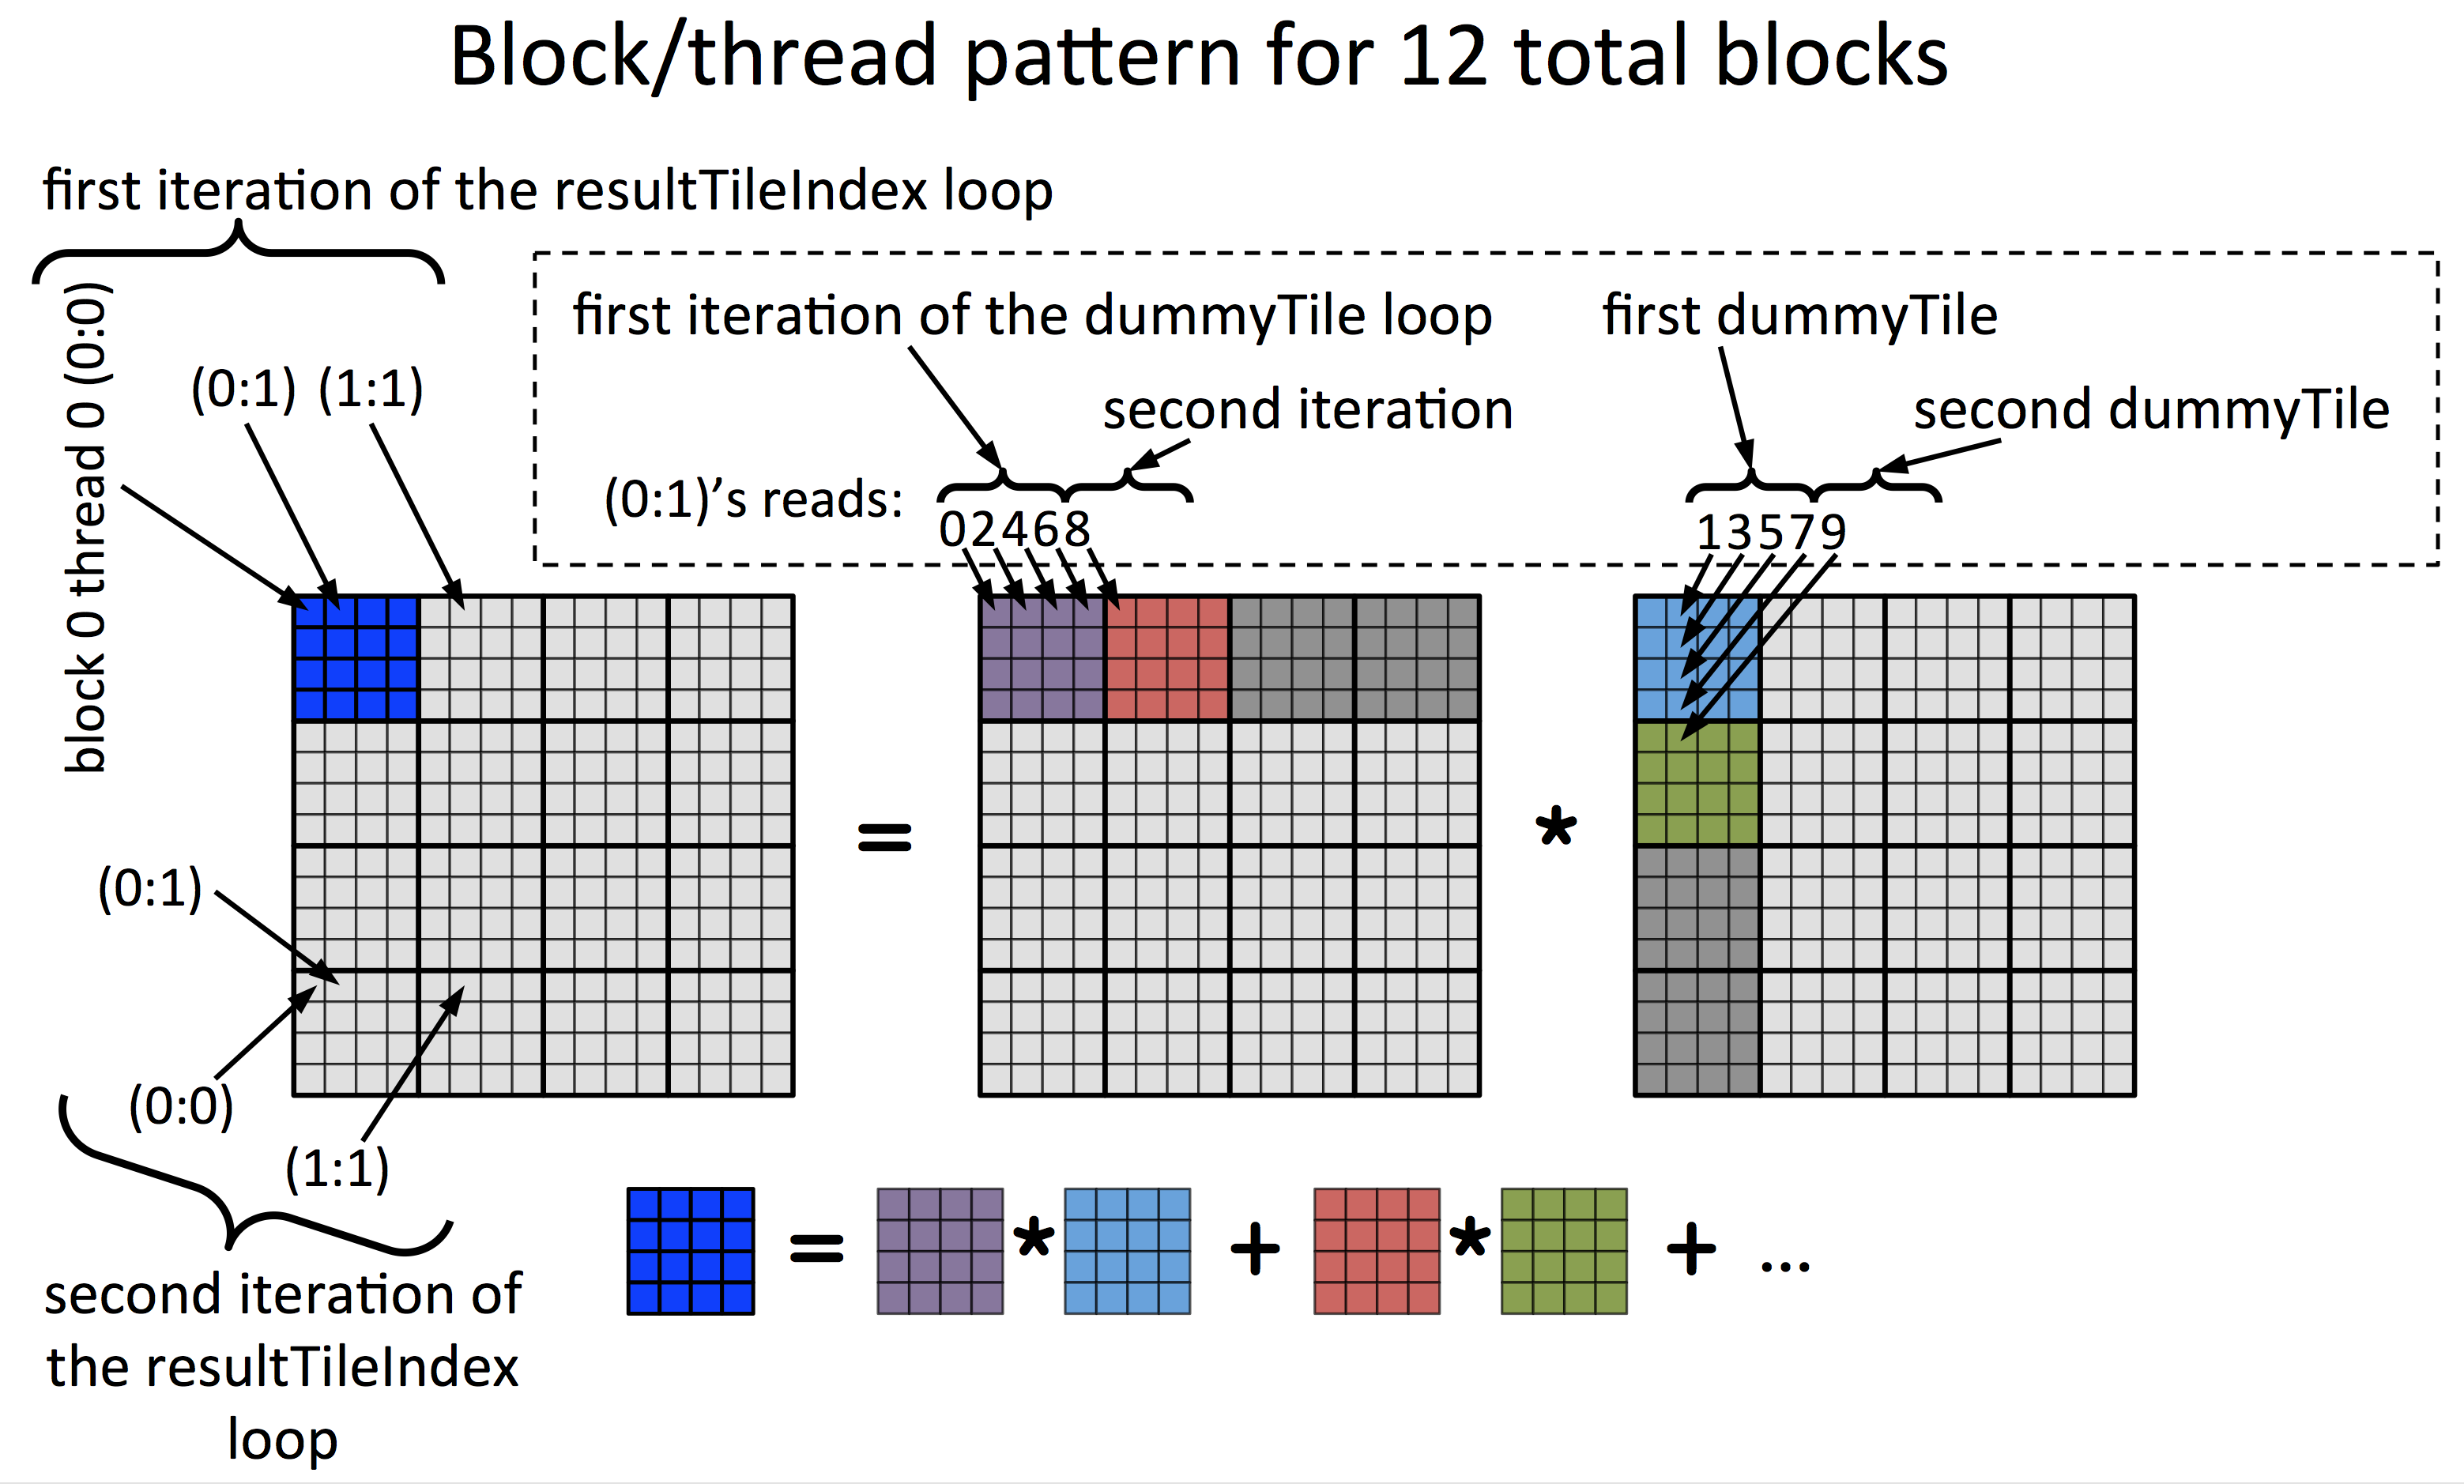
\includegraphics[width=5.0in]{tiled_blocks_threads}
\end{center}

Below you'll find a plot of the speedup (compared to serial CPU) of all of these versions.  
How good is your best version compared to \texttt{cublas}?  
Comment on your results.

\ifSolutions
\textbf{Solution}

{
  \begin{figure}[h!]
    \begin{center}
    \begin{tabular}{c}
    \subfloat{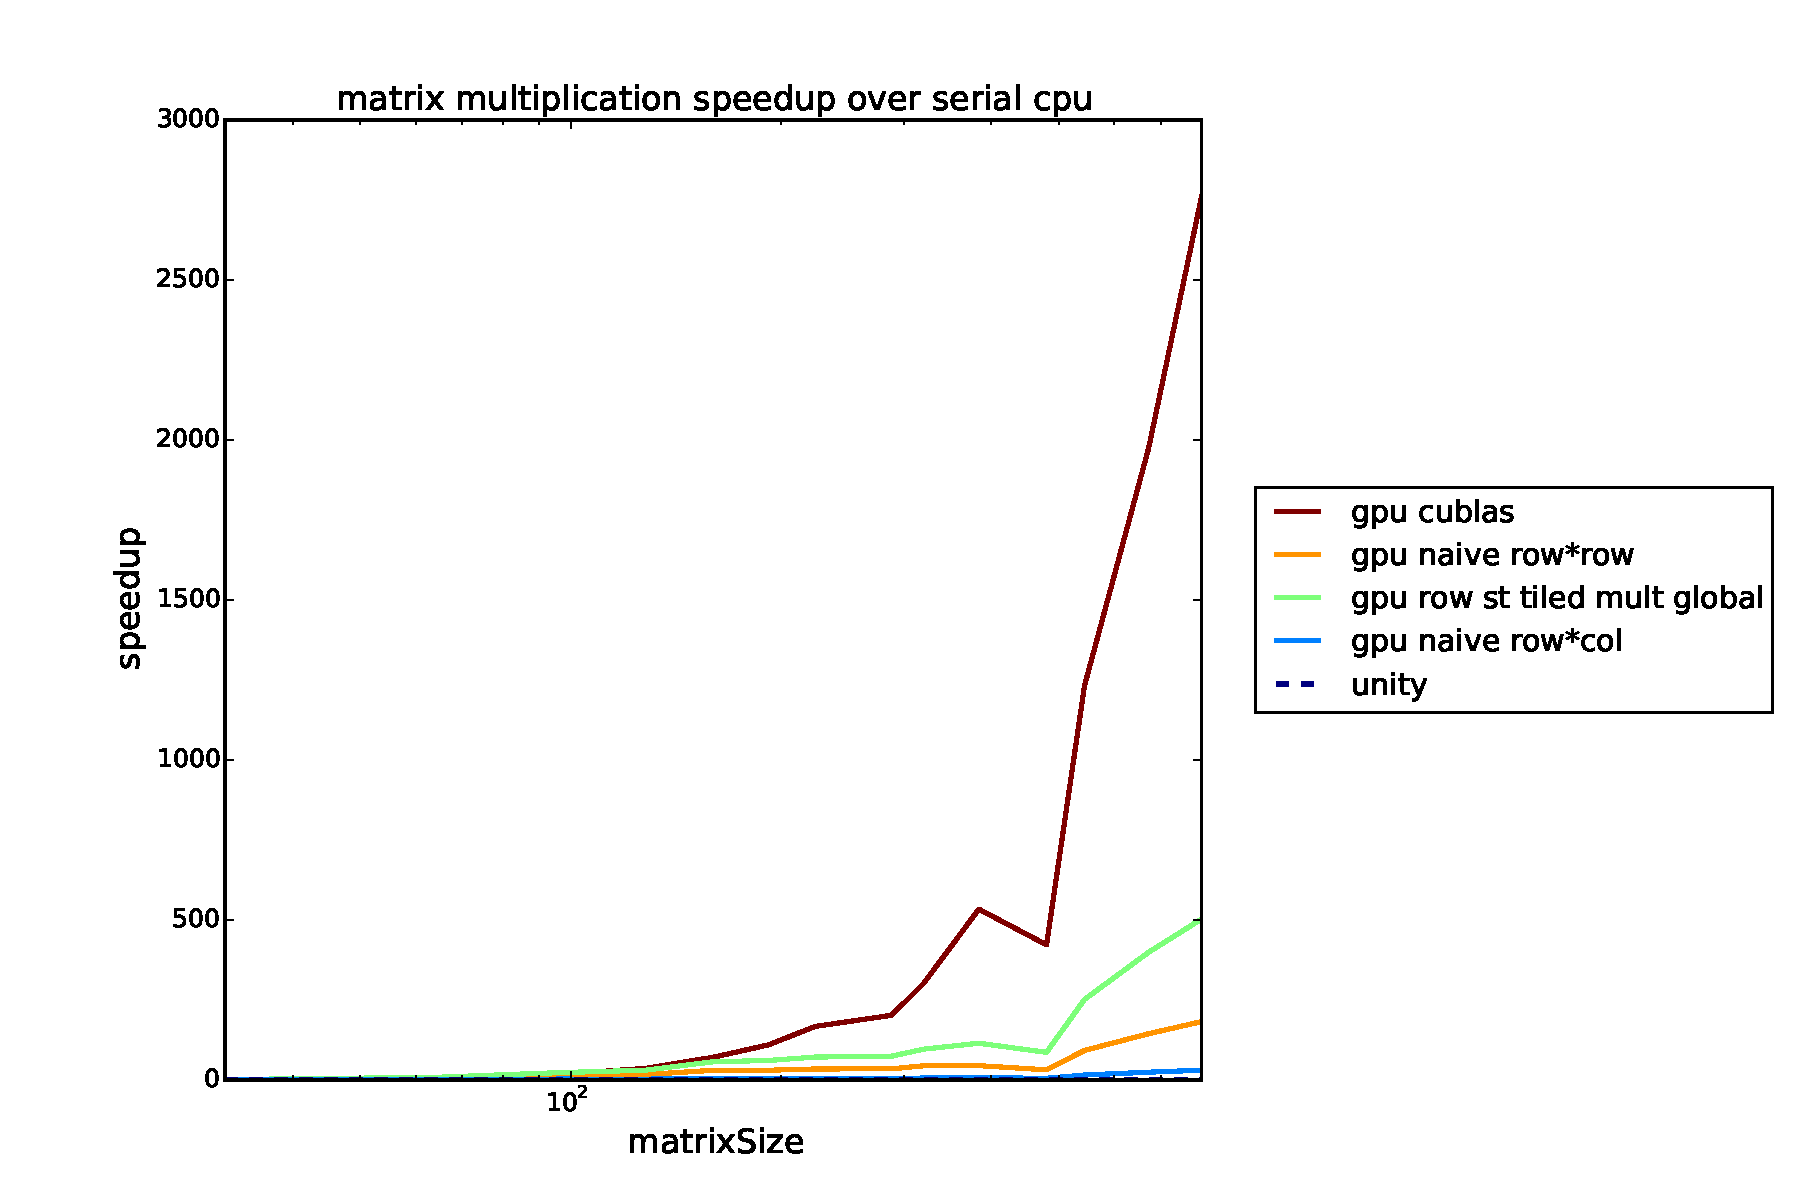
\includegraphics[width=6.0in]{figures/MatrixMultiplication_matrixMultiplication_shuffler}} \\
    \end{tabular}
    \end{center}
    \caption{Performance of matrix multiplication}
    \label{fig:Main4}
  \end{figure}
}

\fi

\FloatBarrier
\vfill









\eprob{15}{The Great Reduction Race}

GPUs aren't really designed to do reductions (why would you need them to draw triangles?), but the reality is that they're an integral part of many high performance computing applications.  
In this problem, we'll explore the relative performance of different ways of doing reductions and compare our performance against a really neat library called \href{http://docs.nvidia.com/cuda/thrust/#axzz3KKFtexoj}{thrust}.  

You only really need to care about how you do your reductions when the cost of doing the reduction is significant compared to the cost of generating the numbers to reduce, so sometimes it doesn't matter at all how you do the reduction.  
On this problem, we'll simply sum a list of numbers to see performance in the extreme case of not doing any work to generate the numbers, where the reduction performance is very important.


\textbf{Note:} Implement your reduction versions so that they work for any number of threads per block that is a power of 2.  
In other words, you can't assume a specific number of threads per block, but you know it's a power of 2 (256, 512, and 1024, etc.).

\textbf{Note:} No matter which version you're implementing, no thread should do more than one atomicAdd.

\begin{enumerate}[a)]
\item Implement the following two versions:
  \begin{enumerate}[1.]
  \item The \texttt{SerialBlockReduction} version, where all the threads in a block calculate their individual values, load their values into shared memory, then thread 0 sums up all of those values in shared memory and atomically adds that whole block's contribution to the global counter.
  \item The \texttt{Stupendous} version.
  This version can be one of four choices: either the ``divergent tree'' version described on slide ``c = a dot b (9)'', or the ``convergent tree'' version described on slide ``c = a dot b (10)'', or a ``warp synchronous'' version where you rely on the fact that warps do operations in lock-step and you don't use \emph{any} \texttt{syncthreads} calls, or some combination of warp synchronicity and a tree.
\end{enumerate}

You don't need to say anything for this part of the problem, the plots will come next.

\item The provided rendering script generates several plots.  
First, it makes 2D plots of the speedup of the reduction versions versus input size for three specific values for the max number of blocks made: 80, 800, and 8000.  
Comment on these plots, pointing out interesting features and saying why they might exist.  
Among anything else you'd like to point out, specifically consider why performance is worse when more blocks are used.

\ifSolutions
\textbf{Solution:}

{
  \begin{figure}[h!]
    \begin{center}
    \begin{tabular}{c}
    \subfloat[80 blocks]{
\includegraphics[width=4.65 in]{figures/ReductionRace_speedup_shuffler_00080}} \\
    \subfloat[800 blocks]{
\includegraphics[width=4.65 in]{figures/ReductionRace_speedup_shuffler_00800}} \\
    \subfloat[8000 blocks]{
\includegraphics[width=4.65 in]{figures/ReductionRace_speedup_shuffler_08000}} \\
    \end{tabular}
    \end{center}
    \caption{Speedup of various gpu versions versus input size}
    \label{fig:Problem1_versusInputSize}
  \end{figure}
}

\fi

\item Next, the script makes 3D plots of the speedup of your \texttt{Stupendous} versions versus max number of blocks and number of threads per block.
Comment on what you learn from this plot.

\ifSolutions
\textbf{Solution:}

{
  \begin{figure}[h!]
    \begin{center}
    \begin{tabular}{c}
    \subfloat{
\includegraphics[width=4.25in, trim=1.25in .5in .55in 0.40in, clip]{figures/ReductionRace_gpuSpeedups_shuffler}} \\
    \end{tabular}
    \end{center}
    \caption{Speedup of tree gpu version versus number of threads per block and number of blocks}
    \label{fig:Problem1_versusThreadsAndBlocks}
  \end{figure}
}

\fi

\end{enumerate}

\FloatBarrier
\vfill










%\newpage

\eprob{20}{Back to the Real World}

Provide short (but sufficient) answers to the following prompts:

\begin{enumerate}[a)]
\item Explain as you would to a ``non-technical'' friend of yours what a GPU is (at a high level, not about warps and such, that's next) and why people other than video game engine makers care about GPUs.

\ifSolutions
\textbf{Solution}

\fi

\item Explain as you would to a ``non-technical'' friend of yours how threads, warps, blocks, streaming multiprocessors, kernels, and GPUs are related.

\ifSolutions
\textbf{Solution}

\fi

\item Explain as you would to a ``non-technical'' friend of yours how a GPU handles the problem of its high memory latency and how it's different from the approach a CPU takes.

\ifSolutions
\textbf{Solution}

\fi

\item Your lab-mate is excited to use a GPU because it has (let's say) 100 or 1000 times more cores on it than their CPU has.  
Your labmate predicts that GPUs will eventually replace CPUs because, come on, it has 100 or 1000 times as many cores.  
What would you tell them to straighten out their confusion?

\ifSolutions
\textbf{Solution}

\fi

\item Answer your CS frosh mentee's (you are mentoring the lower classmembers, right?) inevitable question: ``how do you write a program to use the GPU''?

\ifSolutions
\textbf{Solution}

\fi

\end{enumerate}

\vfill

\eprob{5}{Feedback}

\begin{enumerate}[a)]
\item How much total time did you spend on this assignment?
\item Of the total time, how much total time did you spend ``flailing'' on little annoying things that are not the main point of the assignment?
\item Did you have any ``aha'' moments where something clicked?  If so, on what problems or parts?
\item Can you give me any feedback on this assignment?
\end{enumerate}

\vfill


{\huge\textbf{see the next page for debugging hints}}

\vskip 1cm
\total

\newpage

\section*{Some debugging hints}

\begin{itemize}
\item You can use \texttt{printf} from within kernels, but beware - restrict which threads output or you'll get an enormous flood of messages.
\item Invalid array accesses are hard to track in cuda kernels because the kernel will just crash and silently return.  
One option is to run your program from within \texttt{cuda-memcheck}:

\begin{verbatim}
/usr/local/cuda-7.0/bin/cuda-memcheck ./KMeansClustering
\end{verbatim}

Alternatively, if that's not helpling, you can do something like the following:

\begin{verbatim}
  const unsigned int index = compute an index
#ifdef CUDA_DEBUG
  if (index >= sizeOfArray) {
    printf("bad index = %u under the following conditions:...", index);
    array[0] = -1e7; // or some flag that my cpu code can inspect
    return;
  }
#endif
  array[index] = ...
\end{verbatim}

\end{itemize}




\end{document}

todo: retroactively apply late policy for all students using repository commit times and email them updated grades
